\chapter{Ethereum and Security} \label{ch:security}

The Ethereum platform itself has proven to be robust and reliable as it has been resistant to both censorship and double-spend attacks. In this chapter we discuss vulnerabilities that have been found in the network's implementation which resulted in Denial of Service-like attacks and the blockchain's state being bloated with junk data. Afterwards, we discuss the security of smart contracts and the best practices that need to be applied in order to have a proper workflow. We contribute to the existing literature by evaluating the usage of the tool `Slither' towards finding smart contract vulnerabilities and edge cases. We also improved `Slither' by augmenting the scope of vulnerabilities it was able to detect.
\section{Past Attacks}
\subsection{Network Level Attacks}

\paragraph{October 2016 Spam Attacks}
During the period of September-October 2016, an attacker was able to flood the Ethereum network's state by creating 19 million `dead' accounts. The attack was made possible by a mispricing in the SUICIDE opcode of smart contracts, allowing an attacker to submit transactions that created new accounts at a low cost. The creation of these accounts filled the blockchain's state with useless data which resulted in clients being unable to synchronize in time, effectively causing a \textit{Denial of Service} attack to the network \cite{eip150faq}. As a response, two hard-forks\footnote{A non-backwards compatible upgrade mechanism that creates new rules for a blockchain, usually to improve the system} were proposed \cite{eip607, eip608}. Tangerine Whistle\footnote{EIP608} solved the gas pricing issue and at a later point, Spurious Dragon\footnote{EIP607} cleared the world state from the accounts created by the attack. 

\paragraph{Eclipse Attacks on Ethereum}
\cite{cryptoeprint:2018:236} describes \textit{Eclipse} attacks on Ethereum, a type of attack which by flooding a node's TCP connections is able to make them see a different blockchain history than the network's actual one. This was an attack which was known on Bitcoin which was considered to be harder to perform on Ethereum nodes. The researchers communicated the potential effects of the attack and the vulnerabilities were fixed in geth v1.8\footnote{Most popular implementation of Ethereum in golang}. This vulnerability was not abused in the wild, and as a result there was no need for a hard-fork. It should be noted, that other client implementations such as parity or cpp-ethereum were not found to be vulnerable, which shows that having a diverse set of implementations of a protocol can contribute to the network's security.

\subsection{Smart Contract Attacks}
Contrary to Ethereum as a network, Smart Contracts have proven to be quite vulnerable in the past. We proceed to give a brief description and explanation of the three biggest hacks in Ethereum's Smart Contracts, the `TheDAO' and the `Parity Multisig'\footnote{A multisig is a multisignature cryptocurrency wallet, in this case a smart contract, which requires more than one cryptographic signatures to perform a transaction. It is generally used in organizations and to decrease the chances of funds being stolen. The Parity Multisig refers to a multisig wallet implementation by Parity Technologies, \url{https://www.parity.io/}} (two independent incidents).

\subsubsection{TheDAO} \label{thedao}
TheDAO is an acronym for `The Decentralized Autonomous Organization'. The goal of TheDAO was to create a decentralized business fund where token holders would vote on projects worthy of being funded. TheDAO was initially crowdfunded with approximately \$150.000.000, the largest crowdfunding in history, to date. In July 2016 it was proven that the smart contract governing TheDAO was vulnerable to a software exploit which enabled an attacker to steal approximately 3.600.000 ether, worth more than \$50.000.000 at the time.

If a user did not agree with a funding proposal they were able to get their investment back through the \texttt{splitDAO} function in the smart contract. The function was vulnerable to a \textit{reentrancy}\footnote{Essentially because an account's balance was not reduced before performing a withdrawal it was possible for a malicious user to perform multiple consecutive withdrawals and withdraw bigger amounts than their balance allowed.} attack which allowed an attacker to make unlimited withdrawals from the contract\cite{bloombergdao,hackingdistibuteddao}.

What made TheDAO hack very significant was that as a response, part of the Ethereum community decided to perform a hard-fork to negate the mass theft of funds (~12\% of Ether in existence at the time). This was not accepted by the whole community, and as a result, nodes which did not decide to follow the hard-fork, stayed on the original unforked chain which is still maintained and is called `Ethereum Classic' \cite{etc}. 

\subsubsection{Parity Multisig 1}
In July 2017 a vulnerability was found in the Parity Multisig Wallet which allowed an attacker to steal over 150.000 ether \cite{parityhack}. The attack involved a library contract, which contrary to using Solidity's \texttt{Library} pattern discussed in \ref{method3}, it involves using the \textit{proxy libraries} pattern \cite{proxylibraries} to extract the functionality of a smart contract and let it be usable by other contracts, in order to reuse code, and reduce gas costs, as best practices dictate.

The vulnerability involved the Library contract's \texttt{initWallet} function which was being called through the Parity Multisig Wallet. The function was called when the contract was initially deployed in order to set up the owners of the multisig wallet, however due to it being unprotected it was callable by any user of the wallet\footnote{\url{https://github.com/paritytech/parity/blob/4d08e7b0aec46443bf26547b17d10cb302672835/js/src/contracts/snippets/enhanced-wallet.sol}}. As a result, a malicious user could reinitialize any multisig with their address as the contract's owner and drain its funds.

This was observed by a group of hackers called the `White-Hat Group' who proceeded to drain vulnerable wallets before the attacker could, saving more than \$85.000.000 worth of ether at the time. The unrestricted usage of \texttt{delegatecall} as well as the lack of proper access control on the \texttt{initWallet} function was the cause of this hack. 

\subsubsection{Parity Multisig 2}
After the first Parity hack, a new multisig wallet library was deployed, with access control in the \texttt{initWallet} function. This provided the expected functionality to all Parity Multisig implementations which were using the library. The fix in \texttt{initWallet} involved adding a \texttt{only\_uninitialized} modifier which would only allow modification of the linked multisignature wallet owners during initialization. However, the \texttt{initWallet} function was never called on the library contract itself. As a result, any user could call the \texttt{initWallet} function and set themselves as the owner of the library contract. This alone would not have been dangerous, had there not been a \texttt{kill} function in the smart contract, which when called deletes the contract's bytecode, and effectively renders it useless. 

The attacker\footnote{They claim they were not acting as an adversary.} first became owner of the library by calling \texttt{initWallet} and then proceeded to delete the library by calling the \texttt{kill} function. This resulted in \textbf{all} contracts that were using the library's logic to be rendered useless, effectively \textit{freezing} 513774 Ether, as well as tokens \cite{paritypostmortem}. 

A number of proposals were made \cite{eip867} in order to recover the locked funds. All of these would require an `irregular state change' similar to what happened with the DAO\footnote{~12 million ETH were moved from the “Dark DAO” and “Whitehat DAO” contracts into the WithdrawDAO recovery contract\cite{daofork2}} which was eventually dismissed. 

% https://github.com/paritytech/parity/issues/6995
\section{Evaluating Smart Contract Security}
Due to the high financial amounts often involved with smart contracts, security audits from internal and external parties are considered a needed step before deployment to production. Companies with public smart contracts also engage in bug-bounties, in which they reward users that responsibly disclose vulnerabilities found in their smart contracts. Comprehensive studies on identifying the security, privacy and scalability of smart contracts \cite{DBLP:journals/corr/abs-1710-06372} as well as taxonomies aiming to organize past smart contract vulnerabilities have been done \cite{Atzei:2017:SAE:3080353.3080363,tools}, however due to the rapid evolution of the field they get outdated very soon. 

In order to improve the security of deployed smart contracts, developers must learn to use automated auditing tools and also use the latest version of basic tooling like the Solidity Compiler. As an example, none of the tools mentioned in \cite{tools} were able to detect the `Uninitialized Storage Pointer' vulnerability\footnote{\url{https://github.com/ethereum/solidity/issues/2628}. This particular vulnerability has been exploited in Smart Contract `honeypots' as discussed in Section \ref{honeypots}}, however the Solidity Compiler was later updated to throw a Warning if this issue exists. 

\subsection{Automated Tools}\label{slither}

Auditing smart contracts is significantly more effective when the source code is available. Taking into account the tools which have not been examined in our literature, we came in contact with TrailOfBits, a security auditing firm, and used their suite of tools to extend the already built taxonomies.

We utilized the tool Slither %\footnote{Currently not open-sourced. TrailOfBits shared it with us to use it in the thesis.}
to audit smart contracts. We process all the smart contracts with the latest version of the Solidity compiler, v0.4.22, in order to obtain have access to the latest warnings and errors. 

As Slither is a static analyzer and works on the source code, its modules (called `detectors') are able to find certain coding patterns which can be considered harmful to the smart contract. This includes detecting popular past contract vulnerabilities such as reentrancy or the `Parity bugs', but it is not able to perform symbolic execution and go through all the possible states of a smart contract like Oyente \cite{Luu:2016:MSC:2976749.2978309} or Mythril \cite{mythril}. We describe the currently supported detectors:

\textbf{Constant/View functions that write to state:} Detects \texttt{view} functions that modify a smart contract's state. A \texttt{view} %(\texttt{constant} is deprecated)
function uses the \texttt{STATICCALL} opcode \cite{staticcall} and as a result is unable to modify the state of a smart contract. The latest version of Solidity does not enforce this.

\textbf{Misnamed constructors that allow modification of `owner'-like variables:} A constructor in a smart contract is a function that is named after the contract name and is run once at deployment. It initializes the contract state and usually sets an \texttt{owner} variable which allows the contract owner to have extra administrative permissions on the contract. If a function does not have the same name as the contract then it is callable at any time after deployment. In past cases, constructors were not named properly and were callable by adversaries who would claim ownership of the contract, leading to loss of funds~\cite{Atzei:2017:SAE:3080353.3080363}.

\textbf{Reentrancy bugs:} Due to the TheDAO incident (\ref{thedao}) a lot of attention was raised on reentrancy and race-to-empty\footnote{\url{http://vessenes.com/more-ethereum-attacks-race-to-empty-is-the-real-deal/}} issues and as a result detecting this class of vulnerability is standard in all auditing tools.

\textbf{Deleting a struct with a mapping inside}: Calling \texttt{delete} on a \texttt{struct} object with a \texttt{mapping} variable does not clear the contents of the mapping\footnote{This is warned for in \url{http://solidity.readthedocs.io/en/v0.4.21/types.html}}. This has not been exploited in the wild, however it can be critical in the case of a banking DApp that keeps tracks of balances. A full Proof of Concept is given in \ref{apx:security:mapping}

\textbf{Variable Shadowing:} When a contract (child) that inherits from another contract (parent) defines a variable that already exists in the parent, two separate instances of the variable get stored in the deployed contract. As a result, the parent's (child's) functions can modify only the parent's (child's) state variables. This is currently undetectable by other automated security tools. We further describe how this can get exploited in Section~\ref{honeypots}.

\textbf{Unprotected Function Detection:} If the visibility modifier of a function is set to \texttt{public} or \texttt{external} without any access control mechanism, that function is considered unprotected. This was the cause of the first Parity Wallet hack.

In addition to detecting potential vulnerabilities in smart contracts, Slither's detectors can be used to identify potential code styling issues and recommend fixes:

\textbf{Similar Naming between Variables:} Warns users in the case two variables with same length have very similar names. This is added to encourage more clear and verbose variable naming.

\textbf{Unimplemented Function Detection:} This ensures that the implementation of an interface stays compliant and does not diverge from the intended specification.

\textbf{Unused State Variables:} Detects state variables that are not used in any function and suggests their removal.

\textbf{Wrong Event Prefix:} As per the best practices, the names of `events' should be capitalized. After a discussion on Github\footnote{\url{https://github.com/ethereum/solidity/issues/2877}}, using `emit' for events is going to be mandatory for Solidity 0.5.0 and onwards.

Slither can be used both for finding known vulnerabilities, but also to avoid common anti-patterns. Due to its modular API we can extend it to include more rules. We contributed to the Slither repository by adding support for detecting usage of \texttt{tx.origin} and \texttt{block.blockhash}. The usage of \texttt{tx.origin} should be avoided unless necessary, and as stated in the Solidity documentation can incur in loss of funds\footnote{\url{http://solidity.readthedocs.io/en/v0.4.21/security-considerations.html}}. \texttt{block.blockhash} has been misused in smart contracts and has resulted in amounts up to 400 ETH to be stolen~\cite{smartbillions}. We also contributed to the improvement of the accuracy of the module \texttt{UnimplementedFunctionDetection}. Finally, we implemented a detector to find unassigned calls to a library's functions (calling a library function on a variable does not assign its result back to the variable, it needs to be assigned manually). Table \ref{table:slither} is a modified version of Table 12 from \cite{tools}, including Slither after our contributions, excluding issues that are now detectable by the Solidity compiler. % and excluding any class of vulnerabilities\footnote{Mishandled exceptions, } that can be found by running the latest version of the Solidity compiler.

\begin{table}[htb]
	% \caption{Comparison of vulnerabilities each tool is able to find. Slither is able to detect well known issues along with more subtle ones which are not detectable by other tools. It is not able to recognize Time Order Dependency (TOD) or High Gas cost patterns because they require symbolic execution.}
	\caption{Slither is able to detect more vulnerabilities compared to other tools.}
	\label{table:slither}
	\centering
	\scriptsize
	\setlength\LTleft{-1in}
	\setlength\LTright{-1in}
	\begin{tabular}{|c|c|c|c|c|c|c|}
		\hline
		\textbf{Vulnerability} & 
		\textbf{Oyente} & \textbf{Remix} & \textbf{Securify} & \textbf{SmartCheck} & \textbf{Mythril} & \textbf{Slither} \\ \hline
		\textbf{Reentrancy}        & Y & Y & Y & Y & Y & Y \\
		\textbf{TOD}               & Y & Y & Y & Y & Y & N \\
		\textbf{High Gas}          & N & Y & N & Y & Y & N \\
		\textbf{Unprot. Function}  & N & N & N & N & Y & Y \\  
		\textbf{No Constructor}    & Y & N & N & N & Y & Y \\ 
		\textbf{tx.origin}         & N & Y & Y & Y & Y & Y \\ 
		\textbf{blockhash}         & N & Y & N & N & N & Y \\
		\textbf{Var. Shadowing}    & N & N & N & N & N & Y \\ 
		\textbf{Mapping in struct} & N & N & N & N & N & Y \\ 
		\hline
	\end{tabular}
	\vspace{-2ex}
\end{table}


\subsection{Honeypot Smart Contracts} \label{honeypots}
Since the second Parity bug no novel critical vulnerabilities have been identified in smart contracts. However, smart contracts that are architected to look vulnerable to known exploits started surfacing, when their true purpose is stealing the funds of aspiring hackers. % These contract honeypots are funded with an initial small amount of ether (0.5 to 2 ether). 
Hackers who attempt to exploit them need to first deposit some amount before trying to drain the contract. Each honeypot has a mechanism to prevent the attacker from draining any funds. As a result, only the contract owner is able to withdraw the balance of the contract, including any stolen amounts. % An extensive analysis of smart contracts as honeypots is made in \cite{honeypots} which was released to accompany the research of this Master Thesis. 
We proceed to describe the functionality of a honeypot which takes advantage of `Variable Shadowing' in Solidity. 

The contract in Figure \ref{fig:owner_honeypot} was deployed with an initial amount of 0.1 ether as a balance. At first, it seems that the \texttt{owner} variable can be manipulated by an adversary, by sending ether to the contract with an amount larger than the value of \texttt{jackpot}. After that, the adversary should be able to call \texttt{takeAll} and withdraw the funds from the contract.

\begin{figure}[ht!]
    \centering
    \lstinputlisting[language=Solidity]{contracts/var_shadow.sol}
    \caption{A honeypot which takes advantage of Variable Shadowing.}
    \label{fig:owner_honeypot}
\end{figure}

\begin{figure}[ht!]
    \centering
    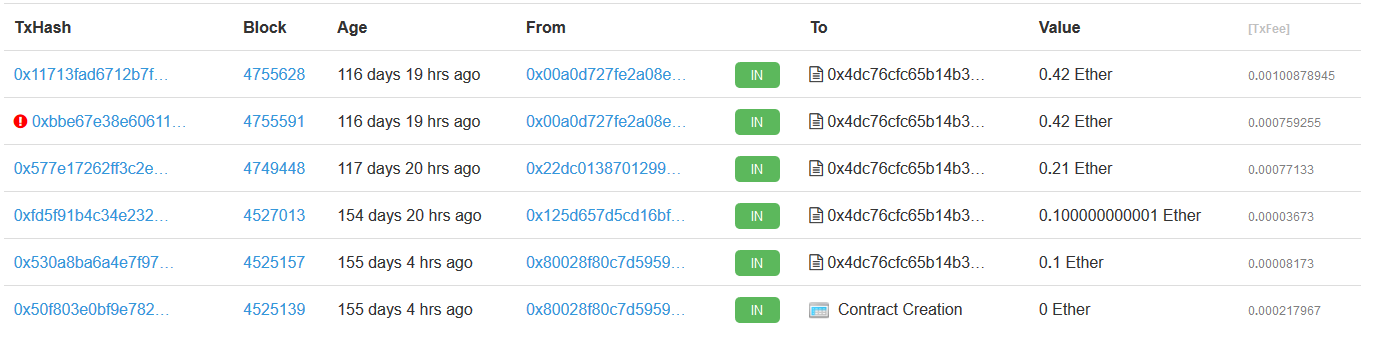
\includegraphics[width=\textwidth]{honeypot}
    \caption{Transactions trying to get ownership of the honeypot contract}
    \label{fig:honeypot_tx}
\end{figure}

Users tried to exploit it by depositing funds and expecting the ownership to change to their address so that they would be able to withdraw the contract's funds. Contrary to what is expected, after sending enough ether to the contract, the \texttt{owner} variable which gets changed belongs to \texttt{KingOfTheHill} contract. The \texttt{takeAll} function, is decorated by the \texttt{onlyOwner} modifier\footnote{A modifier is a special function which gets executed before or after the function it \textit{modifies}. They are primarily used to enforce access control in functions.} which looks for the value of \texttt{owner} in the \texttt{Owned} contract. As a result, the `real' \texttt{owner} of the contract is unchanged, and the attacker is unable to claim ownership, effectively losing their funds. Running Slither on the contract can reveal the variable shadowing as shown in \ref{fig:slither_shadowing}.

\begin{figure}[H]
    \centering
    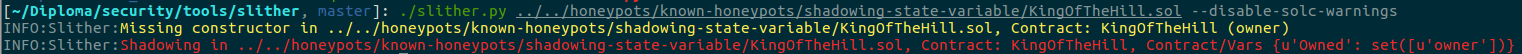
\includegraphics[width=\textwidth]{slither_shadowing}
    \caption{Slither is able to detect the variable shadowing in \texttt{owner}}
    \label{fig:slither_shadowing}
\end{figure}

\subsection{Towards more secure smart contracts}

Trustless smart contracts are impossible to modify after deployment. If a vulnerability is found, it is impossible to patch it. Developers should keep their code as simple as possible, while providing test coverage for as many scenarios as possible. Using audited and tested code for parts of contracts that have already been implemented (e.g. an \texttt{ERC20} token contract) ensures that these parts of the code are going to be secured. Developers must be familiar with the security best practices as described by the industry's most sophisticated auditors\footnote{\url{https://consensys.github.io/smart-contract-best-practices/known_attacks/}}, and should look for confluence between the results of different automated analyzers in order to filter out false-positives and find false-negatives. They should also be testing and improving their skills on platforms that have been set up with intentionally vulnerable contracts \cite{ethernaut, hackthiscontract, capturetheether}. Finally, if compromises in the trustless nature of the contracts can be made, they can be made to be upgradeable, however that increases code complexity, gas costs and potentially introduces new attack vectors.